% MODELO CONEM 2016
\documentclass[10pt,fleqn,a4paper]{article}
\usepackage{abcm}
\begin{document}
    
    % CABEÇALHO
    \fancypagestyle{firststyle}
	{
   		\lhead{\emph{Anais do XXII Encontro de Iniciação Científica e Pós-Graduação do ITA - XXII ENCITA / 2016
	Instituto Tecnológico de Aeronáutica, São José dos Campos, SP, Brasil, 14 de outubro de 2016}}  
	}
    \thispagestyle{firststyle}
    \vspace{-.5cm}
    \hspace{-.8cm}
    \begin{tabular}{p{\textwidth}}
    \begin{center}
    \vspace{-.6cm}
    \title{Controle para Rastreio de Trajetória por um Robô com Acionamento Diferencial Utilizando Retroalimentação por Câmera}
    \end{center}
    \textbf{Téssio Perotti Arruda}\\
    \small{Instituto Tecnológico de Aeronáutica}\\
    \small{Rua H8A, 113, CTA}\\
    \small{12.228-460 - São José dos Campos/SP}\\
    \small{Bolsista PIBIC - CNPq}\\
    \small{tessio.perotti@gmail.com}\\
    \\ 
    \textbf{Carlos César Aparecido Eguti}\\
    \small{Instituto Tecnológico de Aeronáutica}\\
    \small{Centro de Competência em Manufatura}\\
    \small{Praça Marechal Eduardo Gomes, 50}\\
    \small{12.229-900 – São José dos Campos / SP}\\
    \small{cesar.eguti@gmail.com}\\
    \\ 
    \textbf{Marcos Ricardo Omena de Albuquerque Maximo}\\
    \small{Instituto Tecnológico de Aeronáutica}\\
    \small{Divisão de Ciência da Computação}\\
    \small{Praça Marechal Eduardo Gomes, 50}\\
    \small{12.229-900 – São José dos Campos / SP}\\
    \small{maximo.marcos@gmail.com}\\
%    \authors{Nome do primeiro autor, e-mail$^1$} \\
%    \authors{Nome do segundo autor, e-mail$^1$} \\
%    \authors{Nome do terceiro autor, e-mail$^2$} \\\\
%    \institution{$^1$Nome da instituição, endereço para correspondência} \\
%    \institution{$^2$Nome da instituição, endereço para correspondência} \\
%    \\
%    \authors{\textcolor[rgb]{0.98,0.00,0.00}{Mesmo  formato para outros autores e instituições, se houver.}} \\
    \\
    \abstract{\textbf{Resumo:} O propósito destas instruções é servir de modelo para a formatação de trabalhos a serem publicados nos Anais do CONEM 2016. O resumo deve descrever os objetivos, a metodologia e as principais conclusões em não mais de 4000 caracteres. Ele {\bf não deve conter} nem fórmulas ou deduções matemáticas e nem citações bibliográficas. O trabalho completo será publicado nos anais do envento.}\\
    \keywords{\textbf{Palavras-chave:} palavra 1, palavra 2, palavra 3 (até 5) }\\
    \end{tabular}
    

    \section{INTRODUÇÃO}
        
        Os Anais do CONEM 2016 serão publicados online,  com os artigos no formato Adobe$^{\small{TM}}$ PDF.

        Os artigos devem ser rigorosamente formatados de acordo com estas instruções e este arquivo texto pode ser usado como um template por usuários do \LaTeX\ e, em qualquer caso, como um modelo para os usuários de outros processadores de texto.

        Os artigos estão limitados a um máximo de 10 páginas, incluindo tabelas e figuras. O arquivo final em formato pdf não deve exceder 2,5 MB.

        A língua oficial do congresso é o português; entretanto serão aceitos manuscritos em espanhol ou em inglês. Se o trabalho não for escrito em inglês, o autor deverá incluir o título, os nomes dos autores e afiliações, o resumo e as palavras-chave, traduzidos para o inglês, após a lista de referências, no fim do artigo.


    \section{FORMATO DO TEXTO}
        
        O artigo deve ser digitado em papel tamanho A4, usando fonte Times New Roman, tamanho 10, exceto para o título, nomes dos autores, instituição, endereço, resumo e palavras-chave, que têm formatações específicas indicadas acima. Espaço simples entre linhas deve ser usado ao longo do texto.

        O corpo de texto que contém o título deve ser centralizado, em parágrafo com recuo esquerdo de 0,1 cm e marcado com borda esquerda de largura 2$\frac{1}{4}$ pontos.

        O corpo de texto que contém os nomes de autores e de instituições devem ser alinhados à esquerda, em parágrafo com recuo esquerdo de 0,1 cm e marcados com borda esquerda de largura 2 $\frac{1}{4}$ pontos.

        A primeira página deve ter margem superior igual a 5 cm, e todas as outras margens (esquerda, direita e inferior) iguais a 2 cm. Todas as demais páginas do trabalho devem ter todas as suas margens iguais a 2 cm.

        \textbf{\textcolor[rgb]{0.98,0.00,0.00}{NÃO NUMERAR AS PÁGINAS.}}

        \textbf{\textcolor[rgb]{1.00,0.00,0.00}{QUANDO SUBMETER O TRABALHO PELA PRIMEIRA VEZ EM PDF, OS NOMES DOS AUTORES E AFILIAÇÕES DEVEM SER SUPRIMIDOS. INCLUA APENAS O CÓDIGO DO RESUMO, O QUAL FOI FORNECIDO NO E-MAIL DE ACEITAÇÃO DO SEU RESUMO, MANTENDO O ESPAÇO ORIGINAL DESTINADO AOS NOMES DOS AUTORES E AFILIAÇÃO.}}


    \subsection{Títulos e Subtítulos das Seções }

        Os títulos e subtítulos das seções devem ser digitados em fonte Times New Roman, tamanho 10, estilo negrito, e alinhados à esquerda. Os títulos das seções são com letras maiúsculas (Exemplo: \textbf{MODELO MATEMÁTICO}), enquanto os subtítulos só têm as primeiras letras maiúsculas (Exemplo: \textbf{Modelo Matemático}). Eles devem ser numerados, usando numerais arábicos separados por pontos, até o máximo de 3 subníveis. Uma linha em branco de espaçamento simples deve ser incluída acima e abaixo de cada título ou subtítulo.

    \subsection{Corpo do Texto}

        O corpo do texto é justificado e com espaçamento simples. A primeira linha de cada parágrafo tem recuo de 0,6 cm a partir da margem esquerda.

        As equações matemáticas são alinhadas à esquerda com recuo de 0,6 cm.  Elas são referidas como "Eq. (1)" no meio de uma frase, ou "Equação (1)" quando usada no início de uma sentença. Os números das equações são numerais arábicos colocados entre parênteses, e alinhados à direita, como mostrado na Eq. (1).

        Os símbolos usados nas equações devem ser definidos imediatamente antes ou depois de sua primeira ocorrência no texto. \citep{artigoMangaSBAI}

        O tamanho da fonte usado nas equações deve ser compatível com o utilizado no texto. Todos as grandezas físicas devem ter suas unidades expressas no sistema S.I. (métrico).

        \begin{equation}
        \frac{\partial^2 T}{\partial x^2} + \frac{\partial^2 T}{\partial y^2} = 0 \label{equation1}
        \end{equation}

        As tabelas devem ser centralizadas. Elas são referidas por "Tab. 1" no meio de uma frase, ou por "Tabela 1" quando usada no início de uma sentença. A legenda deve ser centralizada e localizada imediatamente acima da tabela. Anotações e valores numéricos nela incluídos devem ter tamanhos compatíveis com o da fonte usada no texto do trabalho, e todas as unidades devem ser expressas no sistema S.I. (métrico). As unidades são incluídas apenas na primeira linha ou primeira coluna de cada tabela, conforme for apropriado. As tabelas devem ser colocadas tão perto quanto possível de sua primeira citação no texto. Uma linha em branco, em espaço simples, deve ser introduzida entre a tabela, seu título e o texto.

        O estilo de borda da tabela é livre. As legendas das Figuras e das Tabelas não devem exceder 3 linhas.

        \begin{table}[ht]
            \begin{center}
                \caption{\textbf{Resultados experimentais para as propriedades de flexão dos materiais MAT1 e MAT2. Valores médios obtidos em 20 ensaios.}}
                    \begin{tabular}{|c|c|c|}
                    \hline
                    Propriedades do compósito       & CFRC-TWILL        & CFRC-4HS         \\
                    \hline
                    Resistência à Flexão  (MPa)     & 209$\pm$ 10       & 180 $\pm$  15    \\
                    \hline
                    Módulo de Flexão  (GPa)         & 57.0 $\pm$ 2.8    & 18.0 $\pm$  1.3  \\
                    \hline
                    \end{tabular}
            \end{center}
        \end{table}

        As figuras deve ser centralizadas. Elas são referenciadas por "Fig. 1" no meio de uma frase ou por "Figura 1" quando usada no início de uma sentença. Sua legenda deve ser centralizada e localizada imediatamente abaixo da figura. As anotações e numerações devem tem tamanhos compatíveis com o da fonte usada no texto, e todas as unidades devem ser expressas no sistema S.I. (métrico). As figuras devem ser colocadas o mais próximo possível de sua primeira citação no texto. Deve ser deixada uma linha em branco, de espaçamento simples, entre as figuras e o texto.
    
        \begin{figure}[h]
            \begin{center}
                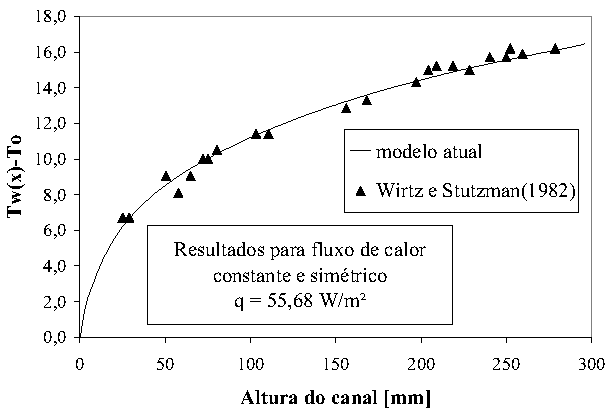
\includegraphics[angle=0, scale=.8]{figura.pdf}
            \end{center}
            \caption{\textbf{Comparação entre os resultados do presente modelo com os resultados experimentais de Wirtz e Stutzman (1982).}}
        \end{figure}

        Figuras coloridas e fotografias de alta qualidade podem ser incluídas no trabalho. Para reduzir o tamanho do arquivo e preservar a resolução gráfica, os arquivos das imagens devem ser convertidos para o  formato GIFF (para figuras com até 16 cores) ou para o formato JPEG (alta densidade de cores), antes de serem inseridos no trabalho.

        A citação das referências no corpo do texto pode ser feita nos formatos: "\citet{Bordalo89} mostra que o corpo...", ou: "Vários trabalhos (\citeauthor{Coimbra78}, \citeyear{Coimbra78}; \citeauthor{Clark86}, \citeyear{Clark86} e \citeauthor{Sparrow80},  \citeyear{Sparrow80}) mostram que a rigidez...".

        
         %   \citet{key} ==>>                Jones et al. (1990)
         %   \citet*{key} ==>>               Jones, Baker, and Smith (1990)
         %   \citep{key} ==>>                (Jones et al., 1990)
         %   \citep*{key} ==>>               (Jones, Baker, and Smith, 1990)
         %   \citep[chap. 2]{key} ==>>       (Jones et al., 1990, chap. 2)
         %   \citep[e.g.][]{key} ==>>        (e.g. Jones et al., 1990)
         %   \citep[e.g.][p. 32]{key} ==>>   (e.g. Jones et al., p. 32)
         %   \citeauthor{key} ==>>           Jones et al.
         %   \citeauthor*{key} ==>>          Jones, Baker, and Smith
         %   \citeyear{key} ==>>             1990
        
        Referências aceitas incluem: artigos de periódicos, dissertações, teses, artigos publicados em anais de congressos, livros, comunicações privadas e artigos submetidos e aceitos (com fonte identificada) e citações a páginas da internet.

        A lista de referências deve ser uma seção específica denominada Referências, localizada no fim do artigo.

        A primeira linha de cada referência deve ser alinhada à esquerda; todas as outras linhas têm recuo de 0,6 cm da margem esquerda. Todas as referências incluídas na lista devem aparecer como citações no texto do trabalho.

        As referências devem ser postas em ordem alfabética, usando o último nome do primeiro autor, seguida do ano da publicação. Exemplo da lista de referências é apresentado abaixo.


    \section{AGRADECIMENTOS}
    
        Se houver, esta seção deve ser colocada antes da lista de referências.


    % REFERÊNCIAS
    \section{REFERÊNCIAS}
        \bibliographystyle{abcm}
        \bibliography{bibliografia}

    \section{RESPONSABILIDADE AUTORAIS}

        Os trabalhos escritos em português ou espanhol devem incluir (após direitos autorais) título, os nomes dos autores e afiliações, o resumo e as palavras chave, traduzidos para o inglês e a declaração a seguir, devidamente adaptada para o número de autores.
    
        O(s) autor(es) é(são) o(s) único(s) responsável(is) pelo conteúdo deste trabalho.

% % RESUMO EM INGLES
%
%\noindent{
%   \\ 
%    \begin{tabular}{||p{\textwidth}}
%    \begin{center}
%    \vspace{-.6cm}
%    \title{AFTER FULL PAPER IN PORTUGUESE OR SPANISH, IT’S NECESSARY THE ABSTRACT IN ENGLISH}
%    \end{center}
%    \authors{First Author’s Name, e-mail1$^1$} \\
%    \authors{Second Author’s Name, e-mail$^2$} \\
%    \authors{Third Author’s Name, e-mail$^2$} \\\\
%    \institution{$^1$Institution and address for first author} \\
%    \institution{$^2$Institution and address for second and third authors} \\
%    \\
%    \authors{\textcolor[rgb]{0.98,0.00,0.00}{Same format for other authors and institutions, if any.}} \\
%    \\
%    \abstract{\textbf{Resumo:} The purpose of these instructions is to serve as a guide for formatting papers to be published in the Proceedings of the IX CONEM.  The abstract should describe the objectives, the methodology and the main conclusions of the paper in less than 4000 characters in a single paragraph.  It should not contain either formulae or bibliographic references. The full paper will be published in the proceedings of the event.}\\
%    \keywords{\textbf{Palavras-chave:} keyword 1, keyword 2, keyword 3 (up to 5 keywords) }\\
%    \end{tabular}
%}

\end{document}